In the simple Texter, the sentence embeddings produced by the embedding block, that capture the sentences' overall meanings, are then passed on to the classification block, as shown in Figure~\ref{fig:4_approach/1_texter/2_simple_model/simple_architecture}, where each of them is pushed through the neural multi-label classifier which consists of a single linear layer. The classification block's pooling layer then combines the sentence-wise classification logits to the entity's logits by averaging them.

\begin{figure}[t]
    \centering
    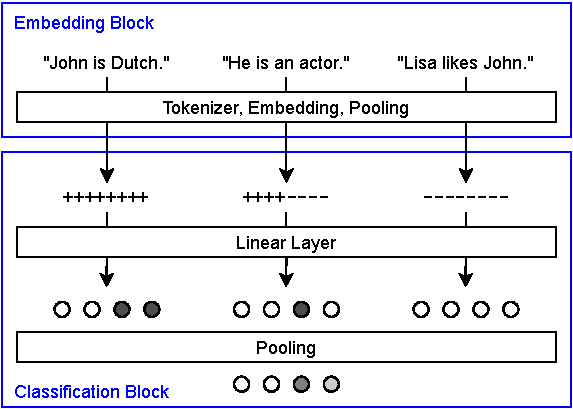
\includegraphics{4_approach/1_texter/2_simple_model/simple_architecture}
    \caption{Simple Texter architecture: Given the sentence embeddings from the embedding block, each sentence is classified individually in the classification block. A pooling layer determines the Texter's output class logits by combining the sentences' class logits.}
    \label{fig:4_approach/1_texter/2_simple_model/simple_architecture}
\end{figure}

Outside the classification block, the sigmoid function is applied to the entity's classification logits, yielding the probabilities for each class. The Texter then derives facts from all classes with a probability greater 50\% by combining the query entity with the relation-tail tuple the classes represent and sorts the predicted facts by confidence. This way, the user gets a list of predicted facts with the most probable ones at the top.
